% XCircuit output "DCL.tex" for LaTeX input from DCL.ps
\def\putbox#1#2#3#4{\makebox[0in][l]{\makebox[#1][l]{}\raisebox{\baselineskip}[0in][0in]{\raisebox{#2}[0in][0in]{\scalebox{#3}{#4}}}}}
\def\rightbox#1{\makebox[0in][r]{#1}}
\def\centbox#1{\makebox[0in]{#1}}
\def\topbox#1{\raisebox{-0.60\baselineskip}[0in][0in]{#1}}
\def\midbox#1{\raisebox{-0.20\baselineskip}[0in][0in]{#1}}
   \scalebox{1}{
   \normalsize
   \parbox{2.83333in}{
   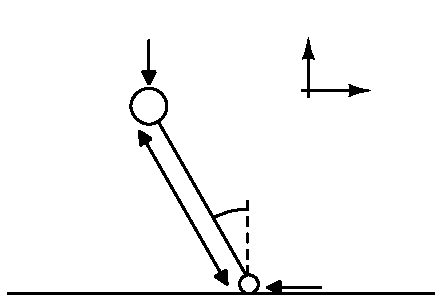
\includegraphics[scale=1]{DCL}\\
   % translate x=512 y=192 scale 0.38
   \putbox{1.16in}{1.31in}{1.20}{\midbox{$m$}}%
   \putbox{2.49in}{1.41in}{1.20}{\midbox{$x$}}%
   \putbox{2.06in}{1.83in}{1.20}{\centbox{$y$}}%
   \putbox{2.14in}{0.16in}{1.20}{\centbox{$F$}}%
   \putbox{0.99in}{1.81in}{1.20}{\centbox{$mg$}}%
   \putbox{1.22in}{0.56in}{1.20}{\rightbox{\midbox{$L$}}}%
   \putbox{1.56in}{0.49in}{1.20}{\centbox{\midbox{$\theta$}}}%
   } % close 'parbox'
   } % close 'scalebox'
   \vspace{-\baselineskip} % this is not necessary, but looks better
